\subsection{Detailed design}
\subsubsection{Diagrams}
\begin{figure}
\centering
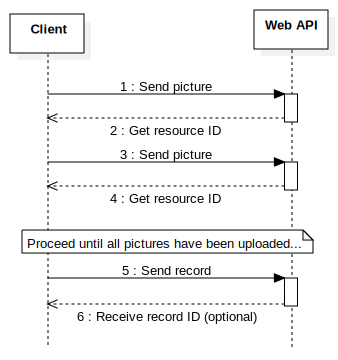
\includegraphics[scale=0.75]{server/SequenceDiagram-AddRecord.svg}
\caption{Sequence diagram: adding a record through the web API}
\label{fig:addRecordSequenceDiagram}
\end{figure}
\subsubsection{Significant data structures}

The web API is going to make use of the Record and Specimen data structures,
which will be exchanged between the server and its clients (the Android
application and the website). They will be represented in a JSON format, which 
is readily available for use in PHP, JavaScript, and Android. Data types, where
specified, are JSON data types.

The structure of a Record is as follows:

Record : Object
    UserName : String
    UserPhone : String
    LocationName : String 
    Specimens : Array of Specimen
    
The structure of a Specimen is as follows:
    
Specimen : Object
    SpeciesName : String
    LocationLatitude : Number
    LocationLongtitude : Number
    Abundance : Number
    Comment : String
    ScenePhoto : String (ID of a resource on the server)
    SpecimenPhoto : String (ID of a resource on the server)